\chapter{Mathematica Code for Kauffman Bound Computation}\label{ch:appendix}

\lstset{language=Mathematica,style=better}

This code is also available as a Mathematica notebook at \cite{my-code}.
Throughout, the pretzel knot $P(a, b, c)$ is encoded by the list \lstinline|{a, b, c}|.

We obtain Lu and Zhong's version of the Dubrovnik Polynomial using the algorithm from \cite{lu-zhong}.
After marking some shorthand and writing out the base change matrix $M$, we directly implement Lu and Zhong's formula for the Dubrovnik polynomial in the function \lstinline|LuZhong[q]|.

\begin{lstlisting}
ai := 1/a;
si := 1/s;
d  := (a - ai)/(s - si) + 1;
di := 1/d;
M   = {
    {   (si - di*si - di*ai) / (s + si),
        (-si - di*s + di*ai) / (s + si),
        di},
    {   (-s - di*si - di*ai) / (s + si),
        (s - di*s + di*ai)   / (s + si),
        di},
    {   (si*d + a - di*si - di*ai) / (s + si),
        (s*d - a - di*s + di*ai)   / (s + si),
        di}
    };

LuZhong[q_] :=
    d * M[[3]] . Table[
        Times @@ (M[[j]] . {s, -si, ai}^#1 &) /@ q, {j, 3}
    ]
\end{lstlisting}

Now we compute the ``standard'' Dubrovnik polynomial, as Lu and Zhong's version has $s - s^{-1}$ instead of $z$ throughout. To do this we need to rewrite the equation in the variables $a, z$ where $z = s - s^{-1}$. This doesn't affect the degree of $a$, but it makes it easier to check that the coefficients of the relevant powers of $a$ are not identically zero.

\begin{lstlisting}
Dubrovnik[q_] := LuZhong[q] /. Solve[z == s - si, s][[1]] // Simplify
\end{lstlisting}

Now we will normalize the Dubrovnik polynomial to get the Kauffman $Y$ polynomial. But first, we need the writhe. For the family we are interested in, the writhe is easy to compute.

\begin{lstlisting}
Writhe[{3, -3, n_}] := -n
Kauffman[q_] := Simplify[Dubrovnik[q] * ai^Writhe[q]]
\end{lstlisting}

As we know, we can use the Kauffman polynomial to get an upper bound on the maximal Thurston-Bennequin number. Using Rutherford's version \cite{rutherford} of Tabachnikov's bound \cite{tabachnikov}, we have

\begin{lstlisting}
TBBound[q_] := (-Exponent[Kauffman[q], a, Max]) // Simplify
\end{lstlisting}

Finally, we can allow Mathematica to crunch the terms:

\begin{lstlisting}[escapeinside={(*}{*)}]
$Assumptions = {n (*$\in$*) Integers};
TBBound[{3, -3, n}]
\end{lstlisting}

and the result is \lstinline|-Max[1, 4 + n]| which is of course $\min\{-1, -4-n\}$ as desired.

Is there any $n$ such that coefficient of $a^{n+4}$ or of $a$ vanishes in the Kauffman polynomial of $P(3, -3, n)$?
It is simple to check that this is not the case, verifying the above expression for $\deg_a$.

\begin{lstlisting}
P = Kauffman[{3, -3, n}] // Expand // PowerExpand // Apart // Expand;
coeff1 = Coefficient[P, a, 1] // FullSimplify
coeffn4 = Coefficient[P, a, n+4] // FullSimplify;
Solve[coeff4n == 0, n]
\end{lstlisting}

On the one hand, \lstinline|coeff1 == 1/z|, which is certainly nonzero. Moreover, \lstinline|coeff4n == 0| only in the following condition, which is not satisfied for any integer constant $n$:
\setmuskip{\thinmuskip}{2mu minus 2mu}
\setmuskip{\medmuskip}{3mu plus 2mu minus 3mu}
\[
    n = \frac{ \ln\left((2 + 16 z^2 + 20 z^4 + 8 z^6 + z^8 + 4 z \sqrt{4 + z^2} + 10 z^3 \sqrt{4 + z^2} + 6 z^5 \sqrt{4 + z^2} + z^7 \sqrt{4 + z^2})/2\right)}{\ln 2 - \ln \left(z (-z + \sqrt{4 + z^2}) - 2\right)}
\]
\begin{figure}[h!]
    \centering
    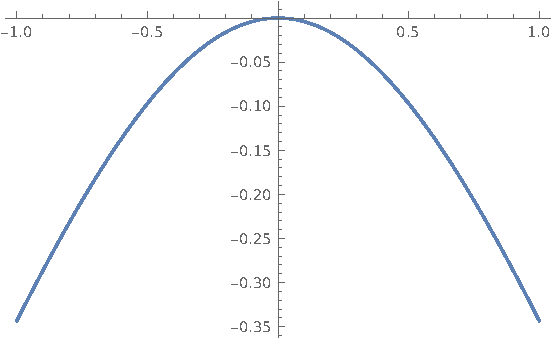
\includegraphics[width=0.3\textwidth]{images/mathematica-n.pdf}
    \caption{A plot of the real part of the above expression, showing that it is not satisfied by any integral constant $n$.}
\end{figure}


